\chapter{Analyse}
Die Analyse untersucht die bestehende Web Applikation und fasst die Anforderungen zusammen. Weiter wird die Struktur der Applikation schematisch dargestellt. Es werden die verwendeten Technologien sowie einen kurzen Exkurs zu anderen Lösungen angesprochen.

\section{Requirements}
Die Anforderungen an die \textit{RadioTour} Applikation ergeben sich aus den Features der bisherigen Web Applikation und den Verbesserungsvorschlägen des \textit{RadioTour} Speakers. Im Anhang \ref{ref:usecases} sind sämtliche UseCases der bisherigen Applikation aufgeführt. Im folgenden Abschnitt werden die Funktionen, welche in diesem Projekt implementiert sind, aufgeführt.

\subsection{Funktionale Anforderungen}
Die funktionalen Anforderungen sind in drei Prioritätsstufen eingeteilt:

\textbf{zwingenden Anforderungen (must)}
\begin{itemize}
\item Fahrerliste, Etappen und Marschtabellen importieren
\item Fahrer ansehen, sortieren und bearbeiten
\item Gruppen bilden und Rückstand angeben
\item Gruppen auflösen
\item Events für Fahrer erfassen (Sturz, Arzt, Aufgabe)
\item Rennsituation an den Server übermitteln
\item Spezialklassemente und Wertungen erstellen und Fahrer zuweisen
\item Maillots erfassen und bearbeiten
\item Persistierung der Daten auf dem Gerät

\end{itemize}


\textbf{optionalen Anforderungen (can)}
\begin{itemize}
\item aktuelle Rennkilometer und Rennzeit anzeigen
\item Stoppuhr
\item aktuelle Position durch GPS bestimmen
\item Events für Fahrer an den Server übermitteln
\end{itemize}


\textbf{wünschenswerten Anforderungen (nice to have)}
\begin{itemize}
\item aktuelle Position des \textit{RadioTour Speakers} in der Marschtabelle anzeigen.
\item \gls{splashscreen} beim Start der Applikation
\item 
\end{itemize}

\subsection{Nicht funktionale Anforderungen}
Im Umfeld eines Live Sport Events spielen neben den funktionalen Anforderungen an ein Software Produkt auch nicht funktionale Anforderungen eine wichtige Rolle. So muss z.B. das UserInterface Fehler bei der Eingabe tolerieren bzw. korrigierbar machen. Die Bedienung muss flüssig verlaufen und zu jedem Zeitpunkt muss der Status der Applikation sichtbar sein. Die für \textit{RadioTour} relevanten nicht funktionalen Anforderungen sind im folgenden aufgelistet.

\begin{itemize}
\item Mobilfunkverbindung ist nicht immer Gewährleistet, keine Daten dürfen dadurch verloren gehen
\item Informationen müssen auch bei direktem Sonnenlicht gut lesbar sein
\item Angenehme, flüssige und selbsterklärende Bedienung der Applikation
\end{itemize}

Weitere nicht funktionale Anforderungen beziehen sich auch auf die Hardware an sich und sind somit im Kapitel \ref{kap:kaufempfehlung} bereits aufgeführt.

\section{Struktur der Applikation}
%ja, plural ist Status, http://de.wikipedia.org/wiki/Status
Die Applikation hat im Grunde zwei Status, einerseits werden vor dem Rennen die Fahrerliste und die Marschtabelle importiert andererseits wird die Rennsituation während dem Rennen erfasst und Änderungen festgehalten. Diese beiden Status können aber nicht absolut voneinander getrennt werden, da während dem Rennen Änderungen denkbar sind. Während dem Rennen müssen gewisse Daten immer angezeigt werden. Diese Live Informationen werden deshalb als eigene Ebene abgebildet. Aus den Anforderungen und den Kriterien entsteht die Baumartige Struktur, wie sie in der Abbildung zu sehen ist.

\begin{figure}[h!]
\caption{Struktur der Applikation als Organigramm}
\centering
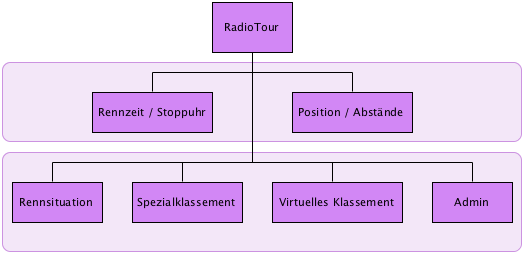
\includegraphics{05bericht/images/struktur.png}
\end{figure} 

Der Stamm stellt die Applikation dar und die Äste zeigen die Aufteilung der Funktionen. Die Rennzeit sowie die aktuelle Rennposition sind in einem immer sichtbaren Bereich platziert.
\\
Die untere Ebene beinhaltet die Kernelemente der Applikation und diese werden in Views seitenweise dargestellt. Durch eine Navigation lässt sich zwischen den Views wechseln ohne, dass dabei die Live Informationen ausgeblendet werden.


\section{Technologien}
\subsection{Android}
Die native Programmiersprache für das Android Betriebssystem ist Java. Die Programmierung in Java bringt den Vorteil, dass auf die gesamte \gls{api} von Android zugegriffen werden kann. Weiter sind die Geräte genau dafür ausgelegt und die optimale Performance kann erreicht werden. Sämtliche Komponenten dieser Arbeit sind in Java geschrieben. Für die Persistierung der Daten auf dem Tablet wird eine \gls{sqlite} Datenbank verwendet.

\subsection{Externe Libraries}
Android beinhaltet bereits ein umfangreiches Framework zur Entwicklung. Deshalb nutzt die \textit{RadioTour} Applikation folgende zwei externe Libraries:
\\
\textit{ORMLite} \footnote{ORMLite, \url{http://ormlite.com/}, Aufgerufen am 23.05.2012} ist eine OpenSource Java Library welche das \gls{orm} übernimmt. ORMLite bietet eine speziell auf Android angepasste Distribution. Um eine Klasse mit ihren Feldern zur Persistierung zu markieren werden Java Annotationen verwendet. Aus diesen Annotationen erstellt ORMLite die Datenbank. Darüber hinaus werden mit ORMLite alle Zugriffe auf die SQLite Datenbank ausgeführt. In dieser Arbeit wird die ORMLite Version 4.39 verwendet.
\\

\textit{Robotium} \footnote{Robotium \url{http://code.google.com/p/robotium/},Aufgerufen am 30.05.2012} ist ein Test Framework welches unter der Apache License 2.0 veröffentlicht und zur freien Nutzung angeboten wird. Robotium untersützt das Testen der Applikation mithilfe von UI Aktionen. In dieser Arbeit wird die version 3.2.1 von Robotium verwendet.  


\subsection{Entwicklungsumgebung}
Die von Android empfohlene Entwicklungsumgebung ist Eclipse\footnote{Eclipse, \url{http://eclipse.org/}} mit einem Plugin zur Entwicklung von Android Applikationen. Auf der Entwicklerseite von Android steht dazu folgendes:
\begin{quote}
\grqq Android Development Tools (ADT) is a plugin for the Eclipse IDE that is designed to give you a powerful, integrated environment in which to build Android applications.\grqq
\footnote{Android Plugin für Eclipse, \url{http://developer.android.com/sdk/eclipse-adt.html}}
\end{quote}
Eclipse ist eine weit verbreitete \gls{ide} und wird aktiv weiter entwickelt. Mit dem Plugin zusammen bilden Sie eine solide Grundlage für dieses Projekt.
\\
Damit die Android Applikation direkt auf dem Computer getestet werden kann, stellt Google ein Emulator zur Verfügung. Der Emulator ist allerdings auch als solcher zu betrachten da die Bedienung nicht vergleichbar ist mit einem richtigen Tablet.

\subsection{Android Version}
Eine Anwendung wird für eine spezifische Android Version entwickelt und getestet, somit kann garantiert werden, dass das Verhalten der Anwendung  immer gleich ist. In dieser Arbeit ist dies die Version 3.1 mit dem Versionsnamen \textit{Honeycomb}.\footnote{\url{Android Version Honeycomb, http://de.wikipedia.org/wiki/Android_(Betriebssystem)\#Versionsverlauf}}.
\\
Die Entwicklung auf einer Version schliesst jedoch nicht aus, dass die Anwendung in neueren Versionen nicht mehr lauffähig ist. Auch \textit{RadioTour} kann für zukünftige Versionen weiterentwickelt und verwendet werden.

\section{Mitbewerberanalyse}
Die Art der Applikation ist sehr spezifisch und kann nicht direkt auf andere Sportereignisse angewendet werden. Deshalb beinhaltet die Analyse von Mitbewerbern nur die grossen europäischen Radrennen. Wie bei der Tour de Suisse ist auch in Frankreich an der \textit{Tour de France}\footnote{Tour de France, \url{http://www.letour.fr/}} ein RadioTour Speaker mit dabei. Darüber wie die Aufzeichnungen in Frankreich im genauen stattfinden kann aber nur spekuliert werden da die Informationen nicht öffentlich zugänglich sind.
\\
In Italien findet zum Zeitpunkt dieser Arbeit der \textit{Giro d'Italia}\footnote{Giro d'Italia, \url{http://www.gazzetta.it/Speciali/Giroditalia/2012/}} statt. Bei diesem Radrennen ist es möglich aus den Informationen, welche auf der Webseite verfügbar sind, zu schliessen, dass ein ähnliches System verwendet wird. Während dem Rennen ist es möglich die aktuelle Rennsituation zu betrachten.

\begin{figure}[h!]
\caption{Rennsituation am Giro d'Italia}
\label{fig:giro}
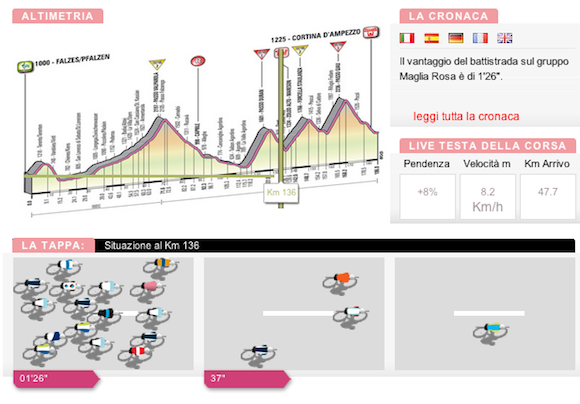
\includegraphics[scale=0.7]{05bericht/images/giro.png}
\end{figure} 

In der Abbildung \ref{fig:giro} ist der Live Abschnitt der offiziellen Webseite zu sehen. Im oberen Teil wird der Standort in der aktuelle Etappe eingeblendet. Weiter unten ist die Situation an der Spitze abgebildet. Die Fahrer sind nach Rückstand gruppiert.
\\
Da jedoch nicht zu erkennen ist, wie die Informationen im Feld erfasst werden, muss die Mitbewerberanalyse an dieser Stelle abgeschlossen werden.